\documentclass[11pt]{article}
% General document formatting
\usepackage[margin=0.75in]{geometry}
\usepackage[parfill]{parskip}
\usepackage[utf8]{inputenc}
\usepackage{subfig}         % side-by-side figures 
% Related to math
\usepackage{amsmath,amssymb,amsfonts,amsthm}
\usepackage{graphicx}
\usepackage{natbib}
\usepackage{titling}
\usepackage{hyperref}
\usepackage{wrapfig}
\usepackage{booktabs} % for wrapping tabulars in accord with
\bibliographystyle{agu}
\setlength{\droptitle}{-5em}   % This is your set screw

%\usepackage[math]{kurier}
\newcommand\be{\begin{equation}} % shortcut to start eq envs 
\newcommand\ee{\end{equation}}   % shortcut to end eq envs
\newcommand\bra{\langle}
\newcommand\ket{\rangle}
\begin{document}

\title{Bedload diffusion theory}
\author{Kevin Pierce}
\maketitle

I consider a two-state random walk with a reaction from one state.
This is a model for alternate motion-rest switching of bedload tracers which can undergo burial when at rest.
Consider un-buried tracers to be a population $A$, while buried tracers are a population $B$.

\begin{wrapfigure}{r}{0.5\textwidth}
	\centering
	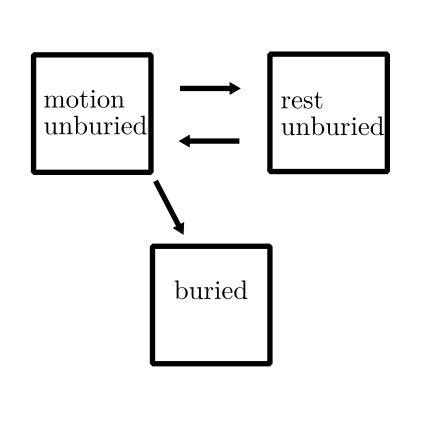
\includegraphics[width=0.5\textwidth,keepaspectratio]{diagram.png}
	\caption{Schematic depiction of the three state process}
	\label{fig:schematic}
\end{wrapfigure}

Let $\omega_2(x,t)$ be the probability that an (unburied) tracer just transitioned into motion having position $x$ at time $t$, and let $\omega_1(x,t)$ be the probability that an unburied tracer just transitioned to rest having position $x$ at time $t$.
Suppose unburied tracers become buried tracers with constant probability $\kappa$ per time.
Then the probability that a resting tracer does not trap by time $t$ is \be\Phi(t) = 1-e^{-\kappa t}.\ee

Let the propagator of a particle through space and time be $g_1(x,t)$ in the rest state and $g_2(x,t)$ in the motion state. These propagators $g_i(x,t)$ characterize the probability that a particle will be found at position $x$ at time $t$ if it started its sojourn in the state $i$ back at $x=0$ and $t=0$.
A key point is that these propagators are asymmetric in space. Particles can only move in the direction of increasing $x$. Hence $g_i(x,t)=0$ for $x<0$.
This reflects the asymmetry of river flow.
\section{Probabilities that a transition just occurred}
Introducting the initial probabilities for a tracer being at rest or in motion as $\theta_1$ and $\theta_2$, and neglecting any possibility that tracers can start ($t=0$) buried, the governing equations can be developed by an argument analogous to that used to develop the multi-state continuous time random walk \citep[e.g.][]{Weiss1994}. The probabilities of being in an unburied state in motion or rest provided a transition just occurred are
\be \omega_1(x,t) = \theta_1 g_1(x,t)\Phi(t) + \int_0^t dt' \int_0^x dx' \omega_2(x',t')g_1(x-x',t-t')\Phi(t-t'), \ee
\be \omega_2(x,t) = \theta_2 g_2(x,t) + \int_0^t dt' \int_0^x dx' \omega_1(x',t')g_2(x-x',t-t').\ee
In the limit of $\kappa \rightarrow 0$ so that no trapping ever occurs, these reduce to the theory of a two state random walk developed by \citet{Weiss1976} and applied to soil transport by \citet{Lisle1998}.

Taking the spatial Laplace transform of the more complicated expression gives
\be \hat{\omega}_1(\eta,t) = \theta_1 \hat{g}_1(\eta,t)e^{-\kappa t} + \int_0^t dt' \hat{\omega}_2(\eta,t')\hat{g}_1(\eta,t-t')e^{-\kappa(t-t')}. \ee
Subsequently taking the temporal transform is more complex but luckily is not so bad because of the trapping-at-constant-rate assumption. Leveraging the Laplace transform shift property \citep[e.g.][]{Arfken1985}:
\be 
\hat{\omega}_1(\eta,s) = \theta_1 \hat{g}_1(\eta, s + \kappa) + \hat{\omega}_2(\eta,s)\hat{g}_1(\eta,s+\kappa)
\ee
\be \hat{\omega}_2(\eta,s) = \theta_2 \hat{g}_2(\eta,s) + \hat{\omega}_1(\eta,s)\hat{g}_2(\eta,s)\ee
These solve for 
\be \hat{\omega}_1(\eta,s) = \frac{\theta_1 + \theta_2 \hat{g}_2(\eta,s)}{1- \hat{g}_1(\eta,s+\kappa) \hat{g}_2(\eta,s)}\hat{g}_1(\eta,s+\kappa)\ee
\be \hat{\omega}_2(\eta,s) = \frac{\theta_2 + \theta_1 \hat{g}_1(\eta,s+\kappa)}{1- \hat{g}_1(\eta,s+\kappa) \hat{g}_2(\eta,s)} \hat{g}_2(\eta,s)\ee
\subsection{Einstein propagators}
Setting $g_1(x,t) = \delta(x)k_1e^{-k_1t}$ and $g_2(x,t) = k_2e^{-k_2 x}\delta(t)$ gives
\be \hat{g}_1(\eta,s+\kappa) = \frac{k_1}{k_1+s+\kappa}\ee
\be \hat{g}_2(\eta,s) = \frac{k_2}{k_2 + \eta}\ee
Starting tracers from rest gives 
\be \hat{\omega}_1(\eta,s) = k_1 \frac{k_2 + \eta}{(k_1 + \kappa + s)\eta + k_2 (s+\kappa)}\ee
\be \hat{\omega}_2(\eta,s) =  \frac{k_1k_2}{(k_1 + \kappa + s)\eta + k_2 (s+\kappa)} \ee

\section{Probabilities away from transition points}
Denoting the probability that a tracer is found unburied and at rest (i.e. in the 1 state) at $x,t$ by $A_1(x,t)$, the probability that it is unburied and in motion (the 2 state) by $A_2(x,t)$, and the probability that it is found buried at $x,t$ by $B(x,t)$, the next equations take the form (need to explain this way better)
\be 
A_1(x,t) = \theta_1 G_1(x,t) \Phi(t) + \int_0^t dt' \int_0^x dx' \omega_2(x',t')G_1(x-x',t-t')\Phi(t-t').\ee 
\be 
A_2(x,t) = \theta_2 G_2(x,t) + \int_0^t dt' \int_0^x dx' \omega_1(x',t')G_2(x-x;,t-t').\ee
I still need to derive the equation for $B(x,t).$
The first two equations can be double transformed for 
\be \omega_1 = \theta_1 g_1\ee


\bibliography{biblio}
\end{document}



